\section{Metodologia}

%\subsection{Equações de fluxo}
%\begin{frame}
%  Em coordenadas radiais, a equação de Richards
%$$
%{\partial \theta \over \partial t} = {1 \over r}{\partial \over \partial r} \left( r K(h) {\partial H \over \partial r} \right)
%$$
%
%e a Equação de Convecção-Dispersão
%
%$$
%r {\partial(\theta C) \over \partial t} = -{\partial \over \partial r} \biggl(r q C \biggr) + {\partial  \over \partial r} \left( r D {\partial C \over \partial r} \right).
%$$
%
%\end{frame}

\subsection{Descrição geral do modelo}
\begin{frame}\frametitle{Características do domínio}

  \begin{tabular}{cl}  
  \begin{tabular}{c}
    \includegraphics[height=2.5cm]{root_zone}\\
    \includegraphics[height=4cm]{domain}
  \end{tabular} &
    \begin{tabular}{l}
    \parbox{0.5\linewidth}{%  change the parbox width as appropiate
      \scriptsize{
	Equação de Richards
	$$
        {\partial \theta \over \partial t} = {1 \over r}{\partial \over \partial r} \left( r K(h) {\partial H \over \partial r} \right)
        $$
	Equação de Convecção-Dispersão
        $$
        r {\partial(\theta C) \over \partial t} = -{\partial \over \partial r} \biggl(r q C \biggr) + {\partial  \over \partial r} \left( r D {\partial C \over \partial r} \right) \\
        $$}

	Condições de contorno em $r_0$:

    \tiny{
      Água:
      $$ K(h) {\partial h \over \partial r} = q_0 = {T_p \over 2 \pi r_0 R z}$$
      Soluto:
      $$ -D(\theta) {\partial C \over \partial r} + q_0 C_0 = q_{s_0} = -{F \over 2\pi r_0 R z}$$
    }

      }
  \end{tabular} 
\end{tabular}
\end{frame}

\begin{frame}\frametitle{Condição de cotorno em $r_0$}

\begin{tabular}{cl}  
  \begin{tabular}{c}
    \centering
    \includegraphics[height=3.5cm]{MM_c}
  \end{tabular} & 
  \begin{tabular}{l}
    \parbox{0.4\linewidth}{ Extração de soluto dependente da concentração de soluto no solo (MM equation) }
  \end{tabular}  \\
  \begin{tabular}{l}
  \parbox{0.5\linewidth}{%  change the parbox width as appropiate
    $$
      F =
      \begin{cases}
	\displaystyle{I_m C_0 \over K_m+C_0}+q_0 C_0, 	&{\rm if }\; C_0 < C_{lim} \\
	I_m, 				 		&{\rm if }\; C_{lim} \leq C_0 \leq C_2 \\
	q_0 C_0, 					&{\rm if }\; C_0 > C_2
      \end{cases}
    $$
  }
  \end{tabular} & \\

\end{tabular}

\end{frame}

\subsection{Implementação numérica da ECD}
\begin{frame}
\end{frame}

\subsection{Other solute uptake models}
\begin{frame}
\end{frame}

\subsection{Scenarios}
\begin{frame}
\end{frame}

\subsection{Other analysis}
\begin{frame}
\frametitle{Other analysis}
Sensitivity analysis

Statistical difference
\end{frame}

